\documentclass[12pt,a4paper]{article}
\usepackage[english]{babel}
\usepackage{ucs} 
\usepackage[utf8x]{inputenc}
\usepackage{mivenndiagram}
\usepackage{tikz}
\usetikzlibrary{intersections}
\usetikzlibrary{calc}
%\usepackage{tikz}
\begin{document}
\begin{venndiagram3sets}[labelA={aaa}, labelB={bb}, labelC={ccc}, labelABC={cccc}]
\fillACapBCapC
\end{venndiagram3sets}
%\usetikzlibrary{calc}
%\begin{tikzpicture}[scale=0.8]
%\draw(4,3)circle(5 and 3)node(A){Text A};
%\draw(8,6)circle(5 and 3)node(B){Text B};
%\draw(10,2.5)circle(5 and 3)node(C){Text C};
%\begin{scope}
%\clip(4,3)circle(5 and 3);
%\clip(8,6)circle(5 and 3);
%\clip(10,2.5)circle(5 and 3);
%\filldraw[yellow!80](0,0)rectangle(10,10);
%\end{scope}
%\node at ($0.33*(A)+0.33*(B)+0.33*(C)$){Text M};
%\end{tikzpicture}
\begin{figure}[h!]
\centering
\begin{venndiagram2sets}[tikzoptions={scale=0.7}]
\fillANotB;
\end{venndiagram2sets}
\end{figure}\\[5pt]
\begin{venndiagram2sets}[labelAB={x}]%%\begin{venndiagram3sets}


\end{venndiagram2sets}%%\end{venndiagram3sets}
\begin{venndiagram3sets}[labelOnlyA={x},labelOnlyB={z,w},labelOnlyC={2}]%%\begin{venndiagram3sets}


\end{venndiagram3sets}%%\end{venndiagram3sets}
\\[5pt]
\begin{venndiagram2sets}[shadeA=red,labelAB={x}]%%\begin{venndiagram3sets}
\fillA \fillB

\end{venndiagram2sets}%%\end{venndiagram3sets}
\\[5pt]
\begin{venndiagram3sets}[labelAB={x}]%%\begin{venndiagram3sets}
\fillA \fillB
\fillC
\end{venndiagram3sets}%%\end{venndiagram3sets}
\\[5pt]
\begin{venndiagram3sets}[tikzoptions={scale=0.8,thick}]%%\begin{venndiagram3sets}
\fillACapC

\end{venndiagram3sets}%%\end{venndiagram3sets}
\\[5pt]
\begin{venndiagram3sets}[shade=blue]%%\begin{venndiagram3sets}
\fillANotC

\end{venndiagram3sets}%%\end{venndiagram3sets}
\\[5pt]
\begin{venndiagram2sets}[shadeA=red,labelAB={x}]%%\begin{venndiagram3sets}
\fillAll

\end{venndiagram2sets}%%\end{venndiagram3sets}
\\[5pt]
\begin{venndiagram3sets}[labelAB={x}]%%\begin{venndiagram3sets}
\fillAll

\end{venndiagram3sets}%%\end{venndiagram3sets}
\\[5pt]
\begin{venndiagram3sets}[labelAB={x}]%%\begin{venndiagram3sets}
\fillNotABC 

\end{venndiagram3sets}%%\end{venndiagram3sets}
\\[5pt]
\begin{venndiagram3sets}[labelAB={x}]%%\begin{venndiagram3sets}
\fillOnlyA 

\end{venndiagram3sets}%%\end{venndiagram3sets}
\\[5pt]
\begin{venndiagram3sets}[labelAB={x}]%%\begin{venndiagram3sets}
\fillOnlyB 

\end{venndiagram3sets}%%\end{venndiagram3sets}
\\[5pt]
\begin{venndiagram3sets}[labelAB={x}]%%\begin{venndiagram3sets}
\fillOnlyC 

\end{venndiagram3sets}%%\end{venndiagram3sets}
\\[5pt]
\begin{venndiagram3sets}[labelAB={x}]%%\begin{venndiagram3sets}
\fillNotA 

\end{venndiagram3sets}%%\end{venndiagram3sets}
\begin{venndiagram3sets}[labelAB={x}]%%\begin{venndiagram3sets}
\fillNotB 

\end{venndiagram3sets}%%\end{venndiagram3sets}
\begin{venndiagram3sets}[labelAB={x}]%%\begin{venndiagram3sets}
\fillNotC

\end{venndiagram3sets}%%\end{venndiagram3sets}
\\[5pt]
\begin{venndiagram2sets}[labelAB={x}]%%para dos conjuntos\begin{venndiagram3sets}
\fillNotAorB 

\end{venndiagram2sets}%%\end{venndiagram3sets}
\begin{venndiagram2sets}[labelAB={x}]%%\begin{venndiagram3sets}
\fillNotAorNotB 

\end{venndiagram2sets}%%para dos conjuntos\end{venndiagram3sets}
\begin{center}
\begin{venndiagram3sets}[shadeA=red!80,shadeB=blue!20,shadeC=green!40!black,labelA={D},labelOnlyA={1},labelOnlyB={2},labelOnlyC={3}, labelOnlyAB={4},labelOnlyAC={5},labelOnlyBC={6},labelABC={7}, labelNotABC={8},tikzoptions={scale=0.8,thick,opacity=0.5}]
\fillA \fillB \fillC
%\fillNotABC 
\end{venndiagram3sets}
\end{center}
%%%%%%%%%%%%%%%%%%%%
\def\firstcircle{[name path=firstcircle] (0,0) circle (2cm)}
\def\secondcircle{[name path=secondcircle] (55:2.67cm) circle (2cm)}
\def\thirdcircle{[name path=thirdcircle] (0:3cm) circle (2cm)}

% Now we can draw the sets:
\begin{tikzpicture}
    \draw \firstcircle node[below,name=A] {$A$};
    \draw \secondcircle node [above,name=B] {$B$};
    \draw \thirdcircle node [below,name=C] {$C$};
    \path [ name intersections = {of = firstcircle and secondcircle } ] (intersection-1) -- (intersection-2) node [pos=0.5] {$A \cap B$};
    \path [ name intersections = {of = secondcircle and thirdcircle } ] (intersection-1) -- (intersection-2) node [pos=0.5] {$B \cap C$};
    \path [ name intersections = {of = firstcircle and thirdcircle } ] (intersection-1) -- (intersection-2) node [pos=0.5] {$A \cap C$};
    \node at ($0.33*(B)+0.33*(C)+0.33*(A)$) {$A \cap B \cap C$};
\end{tikzpicture}
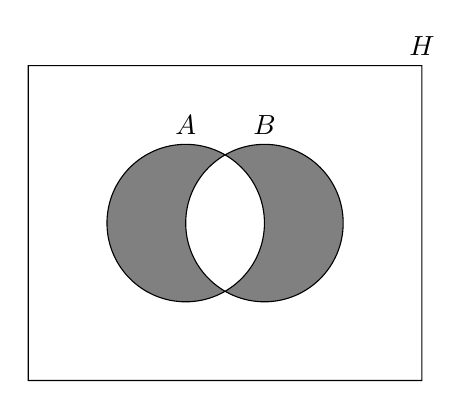
\begin{tikzpicture}[fill=gray]
% left hand
\scope
\clip (-2,-2) rectangle (2,2)
      (1,0) circle (1);
\fill (0,0) circle (1);
\endscope
% right hand
\scope
\clip (-2,-2) rectangle (2,2)
      (0,0) circle (1);
\fill (1,0) circle (1);
\endscope
% outline
\draw (0,0) circle (1) (0,1)  node [text=black,above] {$A$}
      (1,0) circle (1) (1,1)  node [text=black,above] {$B$}
      (-2,-2) rectangle (3,2) node [text=black,above] {$H$};
\end{tikzpicture}
\begin{tikzpicture}[fill=gray]
\node at (4.5,4.6){$U$};
\begin{venndiagram3sets}[labelOnlyA={1},labelOnlyB={2},labelOnlyC={3},
labelOnlyAB={4},labelOnlyAC={5},labelOnlyBC={6},labelABC={7},
labelNotABC={8}]
\fillA
\fillB
\fillC
\end{venndiagram3sets}
\end{tikzpicture}\\

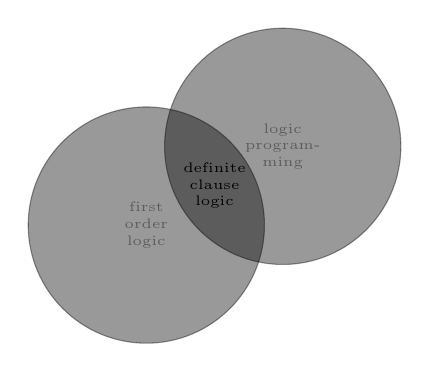
\begin{tikzpicture}[font=\tiny]
  \tikzset{venn circle/.style={draw,circle,minimum width=3cm,
            fill=#1,text width=1cm,align=center,opacity=0.4}%
   }

  \node [venn circle] (A) at (0,0) {first order logic};
  \node [venn circle] (B) at (30:2cm) {logic programming};
  \node[below,text width=1cm,align=center,anchor=center] at (barycentric cs:A=1/2,B=1/2){definite clause logic};
\end{tikzpicture}  


\begin{venndiagram2sets}[shade=blue!20,tikzoptions={scale=0.8,thick}]
\fillA
\fillACapB
\end{venndiagram2sets}

\begin{venndiagram3sets}
\fillACapCNotB
\end{venndiagram3sets}\\
\begin{tikzpicture}[scale=0.8]
\draw(4,3)circle(5 and 3)node(A){Text A};
\draw(8,6)circle(5 and 3)node(B){Text B};
\draw(10,2.5)circle(5 and 3)node(C){Text C};
%\begin{scope}
%\clip(4,3)circle(5 and 3);
%\clip(8,6)circle(5 and 3);
%\clip(10,2.5)circle(5 and 3);
%\filldraw[yellow!80](0,0)rectangle(10,10);
%\end{scope}
%\node at ($0.33*(A)+0.33*(B)+0.33*(C)$){Text M};
\end{tikzpicture}
\begin{venndiagram2sets}[shadeA=red!80,shadeB=red!80,shadeAB=gray,tikzoptions={scale=0.8,thick}]
\fillACapB
\fillA
\fillB

\end{venndiagram2sets}
\end{document}